\documentclass[a4paper]{article}
\usepackage[letterpaper, margin=1in]{geometry} % page format
\usepackage{listings} % this package is for including code
\usepackage{graphicx} % this package is for including figures
\usepackage{amsmath}  % this package is for math and matrices
\usepackage{amsfonts} % this package is for math fonts
\usepackage{tikz} % for drawings
\usepackage{hyperref} % for urls
\usepackage{pdfpages}

\title{Homework 2}
\author{Max Schemitsch}
\date{3/6/2019}

\begin{document}
\lstset{language=Python}

\maketitle

\section{Problem 2.1}
First we can solve the equation for $N$ (and also sub in 0.03 for $\delta$ and 0.05 for $\sigma$.)

\begin{equation}
    \begin{aligned}
\sqrt{\frac{1}{2N}\ln\frac{2M}{0.03}} &\leq 0.05 \\
\frac{1}{2N}\ln\frac{2M}{0.03} &\leq 0.0025 \\
\frac{1}{2}\ln\frac{2M}{0.03} &\leq 0.0025N \\
\frac{\frac{1}{2}\ln\frac{2M}{0.03}}{.0025} &\leq N \\
200 \ln\frac{2M}{0.03} &\leq N \\
    \end{aligned}
\end{equation}

Plugging in $M=1$ gives us $N=840$ samples. \\
Plugging in $M=100$ gives us $N=1761$ samples. \\
Plugging in $M=10000$ gives us $N=2682$ samples. \\

\section{Problem 2.11}
Using this Python code, we can calculate the $E_{out}$ bound with $\delta=0.1$ and for $N=100$ and $N=10000$.

\begin{lstlisting}[frame=single]
import numpy as np
import math
dvc=1
N=100
M=10000
d=0.1

e = math.sqrt(8 / N * np.log((4 * ((2 * N) ** dvc + 1))) / d)
f = math.sqrt(8 / M * np.log((4 * ((2 * M) ** dvc + 1))) / d)
print(e)
print(f)
\end{lstlisting}

\begin{lstlisting}
2.3133697100427275
0.3005306228976483
\end{lstlisting}
Thus our $E_{out}$ bounds for $N=100$, $N=10000$ are roughly 2.3134 and 0.3005 respectively.

\newpage

\section{Problem 2.12}
Using this Python code I borrowed from \\ \url{https://nbviewer.jupyter.org/github/tournami/Learning-From-Data-MOOC/blob/master/Homework\%204.html}, \\
we can calculate the sample size with $\sigma = 0.05$, $\delta = 0.05$ and $d_{vc} = 10$
\begin{lstlisting}[frame=single]
import numpy as np

def get_N(dvc=10, delta=0.05, epsilon=0.05, initial_N=1000, tolerance = 1):
    
    new_N = 8 / epsilon**2 * np.log((4 * ((2 * initial_N)**dvc + 1)) / delta)
    
    if abs(new_N - initial_N) < tolerance: # Did it converge?
        return new_N
          
    else: # If so return N
        return get_N(dvc, delta, epsilon, new_N, tolerance) # Iterate

print("Our sample size must be at least " + format(int(get_N())) + ".")
\end{lstlisting}

\begin{lstlisting}
Our sample size must be at least 452956.
\end{lstlisting}

\newpage

\section{Problem 3.1}
\subsection{A}
We can use the Python code in SemiCircle\_PLA.py to solve part A:

\begin{figure}[h]
  \begin{center}
    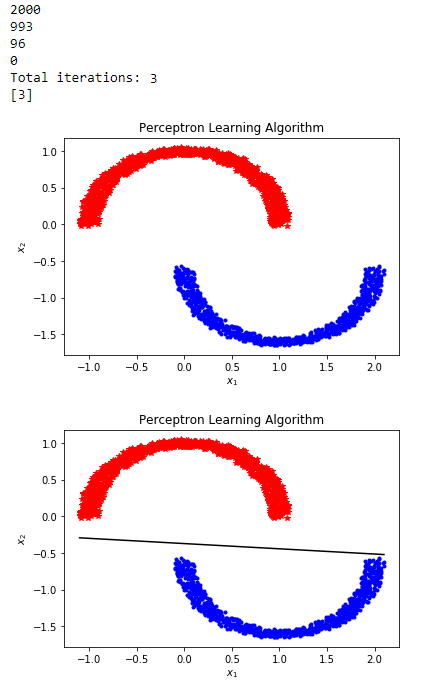
\includegraphics[width=80mm,scale=0.8]{problem3_1a.png}
  \end{center}
\end{figure}

\newpage

\subsection{B}
We can use the Python code in SemiCircle\_Linear.py to solve part B:

\begin{figure}[h]
  \begin{center}
    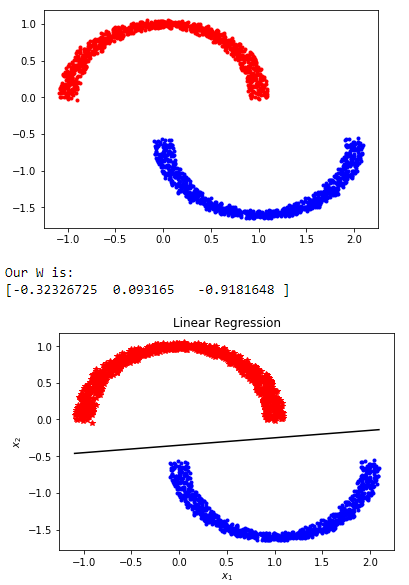
\includegraphics[width=80mm,scale=0.8]{problem3_1b.png}
  \end{center}
\end{figure}

\end{document}